
\documentclass[a4paper,10pt]{article}
\usepackage[a4paper, margin=2cm, voffset=1cm]{geometry}

\usepackage{tikz}
\usetikzlibrary{arrows,calc,shapes,decorations.pathreplacing}
\tikzset{
    vertex/.style = {
        circle,
        fill            = black,
        outer sep = 2pt,
        inner sep = 1pt,
    }
}
\begin{document}
\thispagestyle{empty}
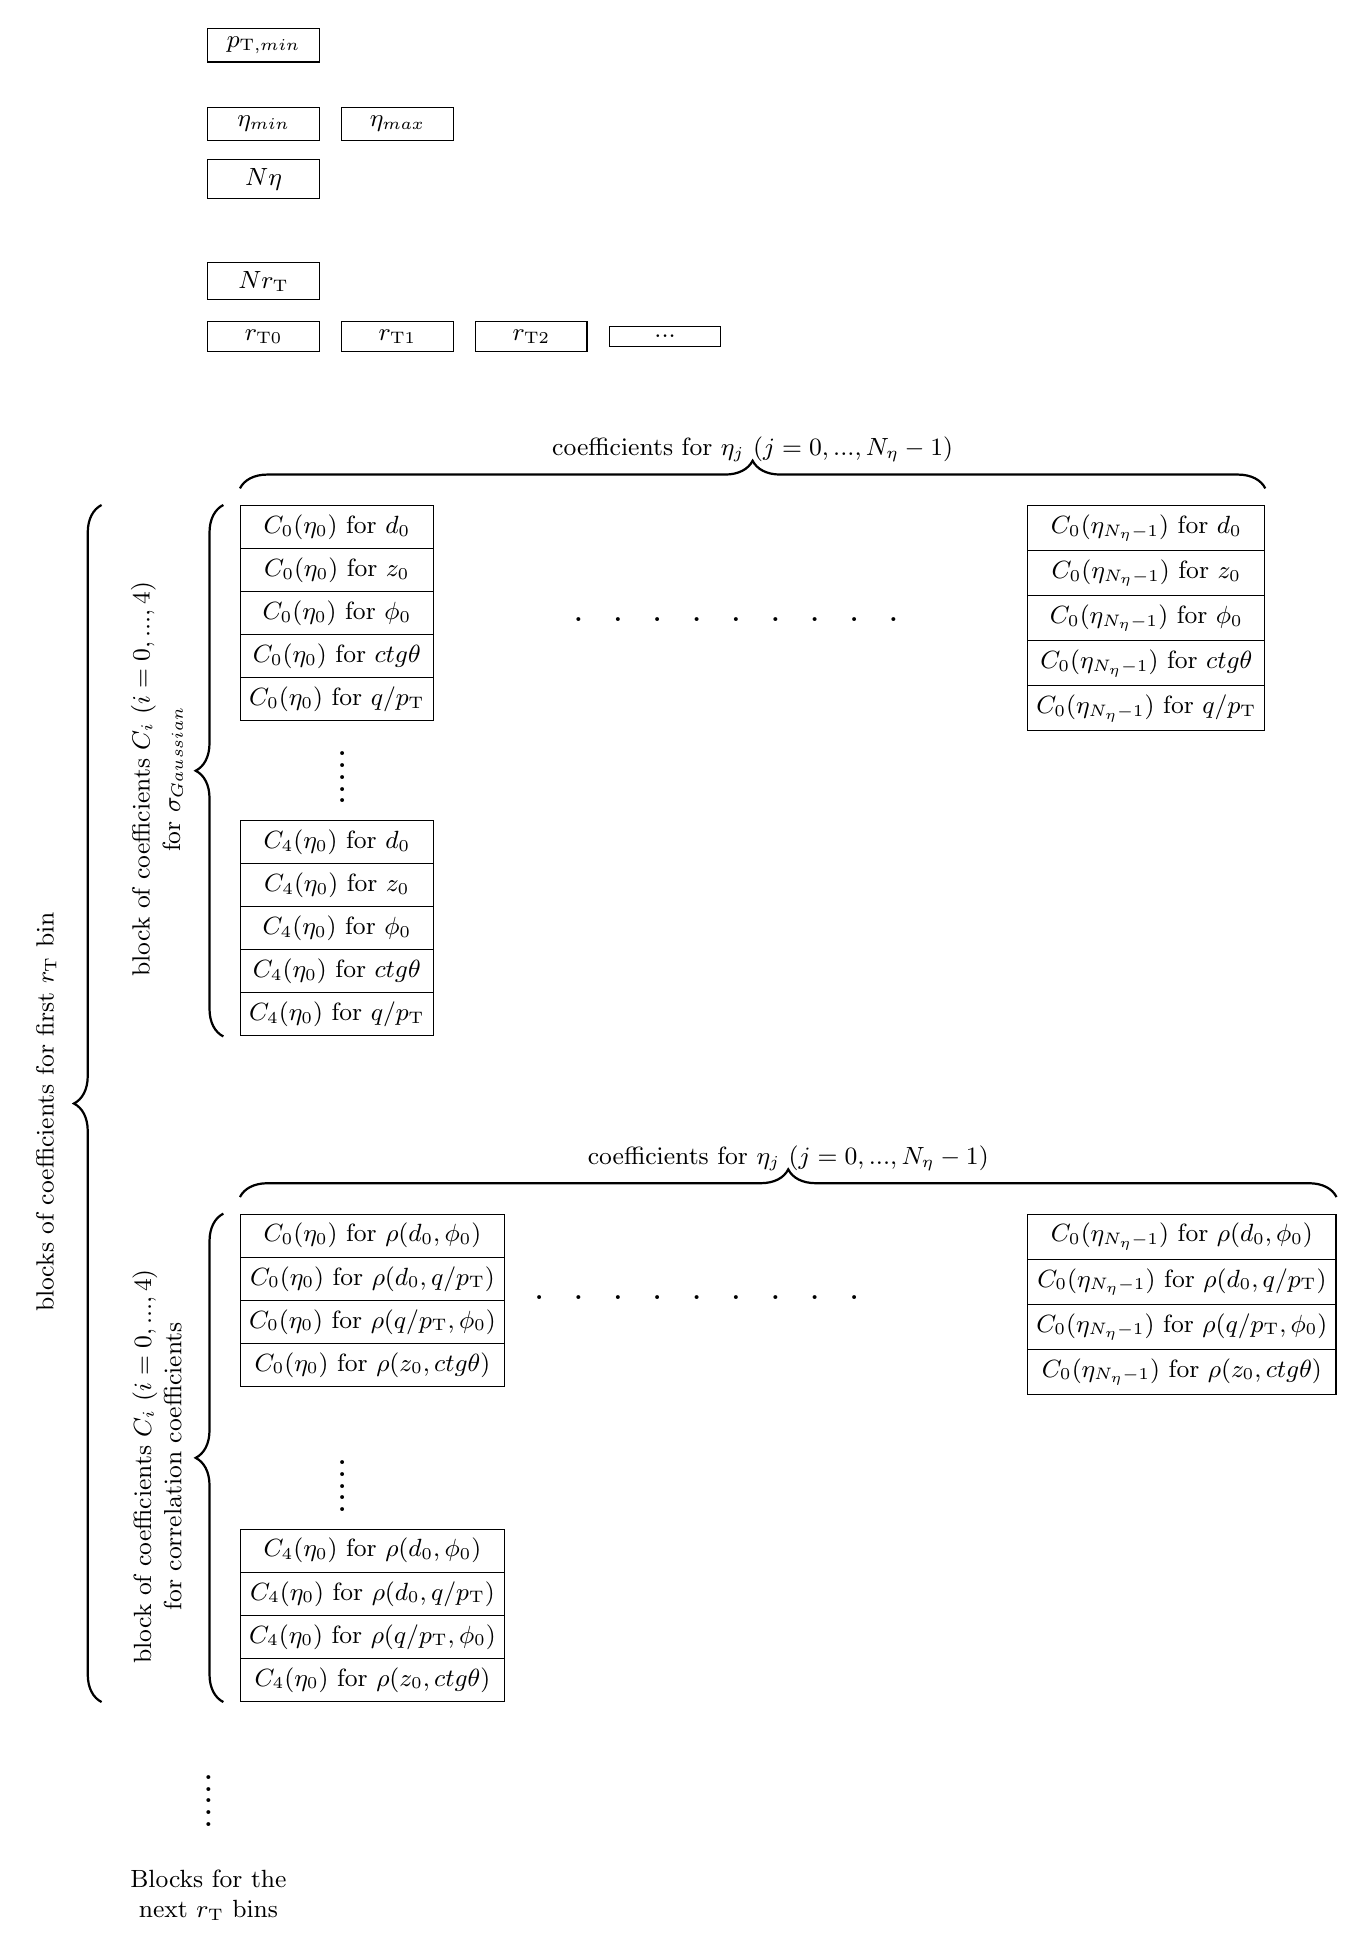
\begin{tikzpicture}
tikzstyle{every node}=[font=\small]


  \node[draw, text width=1.2cm,align=center ] (1) at (0,0) {$p_{\mathrm{T},min}$};
  \node[draw, text width=1.2cm,align=center ] (2) at (0,-1) {$\eta_{min}$};
  \node[draw, text width=1.2cm,align=center ] (3) at (1.7,-1) {$\eta_{max}$};
  \node[draw, text width=1.2cm,align=center ] (4) at (0,-1.7) {$N\eta$};
  \node[draw, text width=1.2cm,align=center ] (5) at (0,-3) {$Nr_{\mathrm{T}}$};
  \node[draw, text width=1.2cm,align=center ] (6) at (0,-3.7) {$r_{\mathrm{T}0}$};
  \node[draw, text width=1.2cm,align=center ] (7) at (1.7,-3.7) {$r_{\mathrm{T}1}$};
  \node[draw, text width=1.2cm,align=center ] (8) at (3.4,-3.7) {$r_{\mathrm{T}2}$};
  \node[draw, text width=1.2cm,align=center ] (9) at (5.1,-3.7) {$...$};


%%%%%%%%%%%%%%%%%%%%%%%%%%%%%%%%%%%%%%%%%%%%%%%%%%%%%%%%%%%%%%%%%%%%%%%%%%%%%%%%%%%%%%%%%%%%%%%%%%%%%%%%%%%%
%% BLOCK FOR GAUSSIAN SIGMA
%%%%%%%%%%%%%%%%%%%%%%%%%%%%%%%%%%%%%%%%%%%%%%%%%%%%%%%%%%%%%%%%%%%%%%%%%%%%%%%%%%%%%%%%%%%%%%%%%%%%%%%%%%%%

  \begin{scope}[every node/.style={draw, anchor=text, rectangle split,
    rectangle split parts=5,minimum width=2.4cm}]
    \node (C0eta0) at (0.,-6.2)
    {
      \nodepart{one} {$C_0(\eta_0)$ for $d_0$}
      \nodepart{two} {$C_0(\eta_0)$ for $z_0$}
      \nodepart{three} {$C_0(\eta_0)$ for $\phi_0$}
      \nodepart{four}  {$C_0(\eta_0)$ for $ctg\theta$}
      \nodepart{five}  {$C_0(\eta_0)$ for $q/p_\mathrm{T}$}
  };
  \end{scope}


  \foreach \y in {0,...,4} {
        \node at (1,-9-0.15*\y) {\bf .};
    }
  \foreach \x in {0,...,8} {
        \node at (4+0.5*+\x,-7.3) {\bf .};
    }


  \begin{scope}[every node/.style={draw, anchor=text, rectangle split,
    rectangle split parts=5,minimum width=2.4cm}]
    \node (C4eta0) at (0.,-10.2)
    {
      \nodepart{one} {$C_4(\eta_0)$ for $d_0$}
      \nodepart{two} {$C_4(\eta_0)$ for $z_0$}
      \nodepart{three} {$C_4(\eta_0)$ for $\phi_0$}
      \nodepart{four}  {$C_4(\eta_0)$ for $ctg\theta$}
      \nodepart{five}  {$C_4(\eta_0)$ for $q/p_\mathrm{T}$}
  };
  \end{scope}


  \begin{scope}[every node/.style={draw, anchor=text, rectangle split,
    rectangle split parts=5,minimum width=2.4cm}]
    \node (C0eta9) at (10.,-6.2)
    {
      \nodepart{one} {$C_0(\eta_{N_{\eta}-1})$ for $d_0$}
      \nodepart{two} {$C_0(\eta_{N_{\eta}-1})$ for $z_0$}
      \nodepart{three} {$C_0(\eta_{N_{\eta}-1})$ for $\phi_0$}
      \nodepart{four}  {$C_0(\eta_{N_{\eta}-1})$ for $ctg\theta$}
      \nodepart{five}  {$C_0(\eta_{N_{\eta}-1})$ for $q/p_\mathrm{T}$}
  };
  \end{scope}

  \draw[decorate,decoration={brace,mirror,raise=6pt,amplitude=10pt}, thick]
    (C0eta0.north west)-- node[left, rotate=90, yshift=30pt, xshift=100pt, align=center, text width=7cm] {block of coefficients $C_i$ (${i=0,...,4}$) \\ for $\sigma_{Gaussian}$ } (C4eta0.south west) ;
  \draw[decorate,decoration={brace,raise=6pt,amplitude=10pt}, thick]
    (C0eta0.north west)-- node[above,yshift=12pt] {coefficients for $\eta_{j}$ ($j=0,...,N_{\eta}-1$)} (C0eta9.north east) ;

%%%%%%%%%%%%%%%%%%%%%%%%%%%%%%%%%%%%%%%%%%%%%%%%%%%%%%%%%%%%%%%%%%%%%%%%%%%%%%%%%%%%%%%%%%%%%%%%%%%%%%%%%%%%
%% BLOCK FOR CORRELATION COEFF
%%%%%%%%%%%%%%%%%%%%%%%%%%%%%%%%%%%%%%%%%%%%%%%%%%%%%%%%%%%%%%%%%%%%%%%%%%%%%%%%%%%%%%%%%%%%%%%%%%%%%%%%%%%%

  \begin{scope}[every node/.style={draw, anchor=text, rectangle split,
    rectangle split parts=4,minimum width=2.4cm}]
    \node (C0eta0_corr) at (0.,-15.2)
    {
      \nodepart{one}{$C_0(\eta_0)$ for $\rho(d_0,\phi_0)$}
      \nodepart{two} {$C_0(\eta_0)$ for $\rho(d_0,q/p_\mathrm{T})$}
      \nodepart{three} {$C_0(\eta_0)$ for $\rho(q/p_\mathrm{T},\phi_0)$}
      \nodepart{four}  {$C_0(\eta_0)$ for $\rho(z_0,ctg\theta)$}
  };
  \end{scope}


  \foreach \y in {0,...,4} {
        \node at (1,-18-0.15*\y) {\bf .};
    }
  \foreach \x in {0,...,8} {
        \node at (3.5+0.5*+\x,-15.9) {\bf .};
    }


  \begin{scope}[every node/.style={draw, anchor=text, rectangle split,
    rectangle split parts=4,minimum width=2.4cm}]
    \node (C4eta0_corr) at (0.,-19.2)
    {
      \nodepart{one}{$C_4(\eta_0)$ for $\rho(d_0,\phi_0)$}
      \nodepart{two} {$C_4(\eta_0)$ for $\rho(d_0,q/p_\mathrm{T})$}
      \nodepart{three} {$C_4(\eta_0)$ for $\rho(q/p_\mathrm{T},\phi_0)$}
      \nodepart{four}  {$C_4(\eta_0)$ for $\rho(z_0,ctg\theta)$}
  };
  \end{scope}


  \begin{scope}[every node/.style={draw, anchor=text, rectangle split,
    rectangle split parts=4,minimum width=2.4cm}]
    \node (C0eta9_corr) at (10.,-15.2)
    {
      \nodepart{one}{$C_0(\eta_{N_{\eta}-1})$ for $\rho(d_0,\phi_0)$}
      \nodepart{two} {$C_0(\eta_{N_{\eta}-1})$ for $\rho(d_0,q/p_\mathrm{T})$}
      \nodepart{three} {$C_0(\eta_{N_{\eta}-1})$ for $\rho(q/p_\mathrm{T},\phi_0)$}
      \nodepart{four}  {$C_0(\eta_{N_{\eta}-1})$ for $\rho(z_0,ctg\theta)$}
  };
  \end{scope}

  \draw[decorate,decoration={brace,mirror,raise=6pt,amplitude=10pt}, thick]
    (C0eta0_corr.north west)-- node[left, rotate=90, yshift=30pt, xshift=100pt, align=center, text width=7cm] {block of coefficients $C_i$ (${i=0,...,4}$) \\ for correlation coefficients } (C4eta0_corr.south west) ;
  \draw[decorate,decoration={brace,raise=6pt,amplitude=10pt}, thick]
    (C0eta0_corr.north west)-- node[above,yshift=12pt] {coefficients for $\eta_{j}$ ($j=0,...,N_{\eta}-1$)} (C0eta9_corr.north east) ;


%%%%%%%%%%%%%%%%%%%%%%%%%%%%%%%%%%%%%%%%%%%%%%%%%%%%%%%%%%%%%%%%%%%%%%%%%%%%%%%%%%%%%%%%%%%%%%%%%%%%%%%%%%%%
%% THE R_T BINS
%%%%%%%%%%%%%%%%%%%%%%%%%%%%%%%%%%%%%%%%%%%%%%%%%%%%%%%%%%%%%%%%%%%%%%%%%%%%%%%%%%%%%%%%%%%%%%%%%%%%%%%%%%%%

  \foreach \y in {0,...,4} {
        \node at (-0.7,-22-0.15*\y) {\bf .};
    }
    \node[text width = 3cm, align=center] (otherRT) at (-0.7,-23.5) {Blocks for the next $r_\mathrm{T}$ bins};



  \draw[decorate,decoration={brace,mirror,raise=50pt,amplitude=10pt}, thick]
    (C0eta0.north west)-- node[left, rotate=90, yshift=70pt, xshift=100pt, align=center, text width=7cm] {blocks of coefficients for first $r_\mathrm{T}$ bin} (C4eta0_corr.south west);


\end{tikzpicture}
\begin{tikzpicture}[overlay]
  \node[text width=20cm, align=left] at (10,25.5) {\bf Example data file \\(based on Atlfast/AtlfastAlgs/AtlfastAlgs-00-05-09/atlfastDatafiles/Atlfast\_MuonResParam\_CSC.dat)};
\end{tikzpicture}
\end{document}
